%File: formatting-instruction.tex
\documentclass[letterpaper]{article}
\usepackage{aaai}
\usepackage{times}
\usepackage{helvet}
\usepackage{courier}
\usepackage{url}
\usepackage[pdftex]{graphicx}
\usepackage{amsmath}
\usepackage{latexsym}
\usepackage{amssymb}
\usepackage{multirow}
\newtheorem{definition}{Definition}
\frenchspacing
\setlength{\pdfpagewidth}{8.5in}
\setlength{\pdfpageheight}{11in}
\pdfinfo{
/Title (From Topics to Opinions: Modeling Subjectivity for Diffusion Behavior Analysis)
/Author (Songxian Xie, Jintao Tang, Ting Wang, Ruili Wang)}
\setcounter{secnumdepth}{0}  
 \begin{document}
% The file aaai.sty is the style file for AAAI Press 
% proceedings, working notes, and technical reports.
%
\title{From Topics to Opinions:: \\Modeling Subjectivity for Diffusion Behavior Analysis}
%\author{Songxian Xie, Jintao Tang \and Ting Wang\\
%School of Computer, National University of Defense Technology, Changsha, P.R. China\\
%\AND Ruili Wang\\
%School of Engineering and Advanced Technology, Massey University, Auckland, New Zealand\\
%\AND Kewen Wang\\
%School of Information and Communication Technology, Griffith University, Brisbane, QLD 4111 Australia\\
%}
\nocopyright
\maketitle
\begin{abstract}
\begin{quote}
Information diffusion plays an important role for both researches and applications in current ``word of mouth'' web. In this paper, we investigate how users' subjectivity influences their information diffusion behavior. 
Inspired by the psychological research, we define a general subjectivity model by combining both topics and opinions articulated in User-Generated Content (UGC) and propose an efficient framework to establish the subjectivity model. 
In order to evaluate the impact of subjectivity on information diffusion behavior, a novel subjectivity similarity measurement between two subjectivity models is put forward.The proposed model has been used to predict the retweeting  behavior on Twitter, by considering the subjectivity similarities in the attractiveness, sociality and popularity aspects. In the experiments, with a statistical hypothesis test and case study, we demonstrate that a user is more likely to retweet a message in terms of the influence of subjectivity. The evaluation on the practical Twitter dataset shows that our  model can improve the performance of retweeting prediction, compared with the state-of-the-art methods.
\end{quote}
\end{abstract}

\section{Introduction}
\label{introduction}
\noindent Information diffusion plays an important role in scenes such as marketing and election by triggering and cascading a large number of users. It has drawn considerable attentions from researchers, especially in the area of online social networks. They have built standard models for the general information diffusion, which are useful for simulating the information flow\cite{goldenberg2001talk,kempe2003maximizing}, or detecting the outbreak of information cascades\cite{cheng2014can}. However, they ignore the intention of users in the process of information diffusion. As information consumer and producer in the web 2.0 era, each user can declare his interests, express opinions, choose information to read and spread on various social media platforms. Whether a message will be spread across the network depends on the ``word of mouth'' effect, which can elicit the diffusion behavior of users. With the development of Natural Language Processing and data mining techniques, the intention of users can be analyzed by modeling users with user-generated data. In this work, we target at an interesting problem: the mechanism of ``word of mouth'' effect, i.e. given a new message from a specific user, we intend to predict who will participate in the future diffusion process after receiving this message. 
As a special scene, we illustrate the problem in a heterogeneous network of Twitter in Figure~\ref{fig00}, in which Tony and his friends have tweeted on two topics: cellphone ``Iphone'' and movie ``Frozen''. Now Tony posts a new tweet about ``Frozen'', we want to find out who will disseminate it among all his friends.
\begin{figure}[htb]
\centering
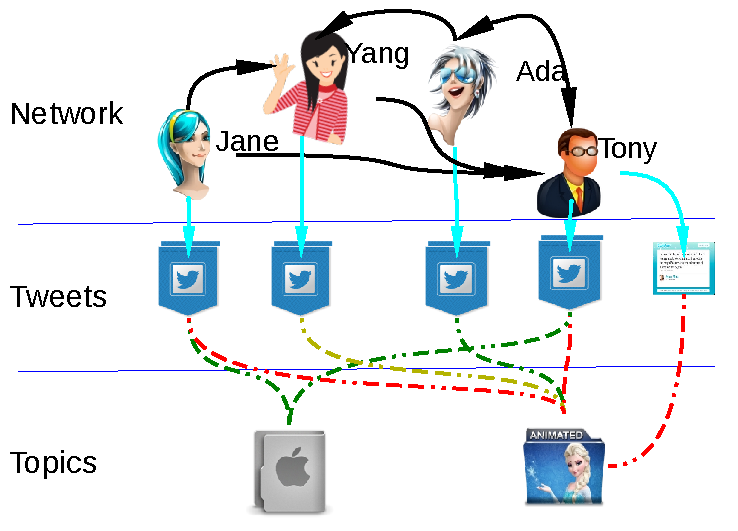
\includegraphics[width=2.2in,height=1.5in]{Mexample.pdf}
\caption{Problem illustration. For opinions of different users, the color ``red'' stands for positive evaluation, ``green'' for negative, and ``yellow'' for neutral.}
\label{fig00}
\end{figure}

The diffusion behavior varies in different social networks. In this paper, we investigate our problem under the context of Twitter, which plays an important role in the process of information diffusion on the Internet because the retweeting convention provides an unprecedented mechanism for the spread of information despite the restricted length of a single message. 
In fact, almost a quarter of the tweets are retweeted from others in Twitter\cite{yang2010understanding}. Therefore, understanding how retweeting behavior works can help explaining information diffusion in Twitter. 

As the participants of information diffusion, users naturally make communication and interaction by expressing opinions and preferences on the topics that interest them. In psychological researches, it has been identified that the subjective initiative nature of human determines that subjectivity will undoubtedly influence his behaviors\cite{moore2008awareness}. According to the theory of Biased Assimilation, people tend to choose and disseminate information according to their own biased opinions\cite{Hyman2000}. Therefore, opinion comprehension is a key aspect of users's intention in the process of information diffusion. 
Previous studies have developed a variety of techniques and models to capture the factors that affect retweeting behaviors\cite{macskassy2011people,feng2013retweet}. However to the best of our knowledge, few studies have investigated the subjective motivation of a user retweeting a message. 
For the  ``word of mouth'' effect in Twitter, retweeting is a process that includes receiving, evaluating and deciding whether to share. The crucial part is to evaluate whether a tweet contains information worthy enough to be shared.  
Therefore modeling the subjective motivation of users will provide an important perspective for retweeting behavior analysis. 
Intuitively, based on the principle of ``like attracts like'', a biased user is prone to retweet a message that meets his own tastes. As for the example in Figure~\ref{fig00}, the tweets of the users have presented their different opinions on two topics. Tony and Jane were positive on movie ``Frozen'', while Ada was negative and Yang was neutral. For the new tweet from Tony which is positive on ``Frozen'', it is easily to understand that Jane is more likely to retweet it because Jane and Tony both like the movie. Therefore how the subjectivity of a user influences his information diffusion behavior is focused on in our work.

For the problem to be investigated, there are two questions arising: how to accurately model the subjectivity of users, and how to effectively measure the worthiness for the users to retweet in terms of subjectivity? 
Answering the questions is non-trivial. 
In this paper, we propose a general method to model subjectivity of users, define a novel similarity measurement to calculate the worthiness,  and identify factors that influence a user's retweeting behavior from the attractiveness, sociality and popularity aspects. 

The rest of the paper is organized as follows: Firstly related works are described; the definition and establishment details of the proposed subjectivity model are given before the subjectivity similarity is defined; Then the factors are specified for the retweeting analysis problem; Further experiments of quantitative evaluation is given; Finally we summarizes the paper and points out future work.

\section{Related Work}
\label{relatedwork}

Sentiment analysis have tried to mine subjective information from reviews\cite{liu2012sentiment}, and there are also many works pay attention to informal text of social media recently\cite{jiang2011target,tan2011user,Guerra2014}. In our work, instead of focusing on opinion in single text piece, we model subjectivity of a user by integrating all opinions scattering in text pieces to his topics of interest. As another line of works similar to our work, topic-sentiment models can also correlate sentiment with topics, for example, TSM~\cite{mei2007topic} model and JST~\cite{lin2009joint} model. Usually they learn a general word-sentiment distribution to model the sentiment of blogs or reviews, and they represent sentiment as binary polarity. Sentiment expression in informal languages is deemed to be more complicated. Sentiment is often embodied in subtle linguistic characteristics such as: misspellings, abbreviations, emphatic uppercasing, emphatic lengthening and the use of slang and neologisms. Moreover, besides polarity,  fine-grained sentiment (strength) is important to distinguish subtle opinions. These lead to much more sparsity in the input and is a special challenge for the word-sentiment distriution. In this paper, we propose to model opinion with a distribution by integrating fine-grained sentiment from a rule-based sentiment analysis method, which can catch subtle sentiment by transforming linguistic characteristics into rules\cite{thelwall2010sentiment}.
   
A large body of studies has analyzed the characteristics of retweeting behavior\cite{Bian2014,Luo:2013RMF}, examining the factors that lead to increased retweetability\cite{suh2010want,comarela2012understanding} and designing models to estimate the probability of being retweeted\cite{jenders2013analyzing,pfitzner2012emotional}. However, all of the above works ignore the subjectivie motivation of users, which is the underlying reason for the retweeting behavior. 

\section{Subjectivity Model}
\label{subjectivemodel}

%Subjectivity has been extensively studied by psychologists to characterize the personality of a person based on his historical behaviors and remarks\cite{engbert2007agency}. 
%Linguists define the subjectivity of language as speakers always show their perspectives, attitudes and sentiments to events, people, topics, and entities in their linguistic contents\cite{stein2005subjectivity}. 
With the explosion of social media over the past decade, more and more User-Generated Content (UGC) is available on the Web containing users' opinions.
In the Natural Language Processing area, opinion mining techniques\cite{liu2012sentiment} have been developed to computationally model the subjectivity of users. A variety of aspect-based or topic-sentiment models have been built from UGC by casting opinions as polarity, ratings, or emotions regarding a topic\cite{lek2013aspect,mei2007topic}. But their utility is often limited by their representation of opinions. In this paper, we give a more general framework to model subjectivity by combining topics and opinions together with a new representation of opinions. Here we give our definition of subjectivity model under context of Twitter, while we emphasize that our model can be adapted to other context as well.

\subsection{Definition}
\label{definition}

Let $G=\left( V,E \right) $ denote a social network on Twitter, where $ V $ is a set of users, and $ E\subset V\times V $ is a set of follow relationships between users. For each user $ u \in V $, there is a tweets collection $ M_{u} $ denoting his message history. We assume that there is a topic space $ T $ containing all the topics that users in $ V $ talk about, and a sentiment space $ S $ evaluating their opinions on these topics. 
For the ``subjectivity'' of a user $ u  \in V $, we refer to both topics and opinions articulated in his tweets collection $ M_{u} $.  
\begin{definition}[Subjectivity Model]
The subjectivity model of user $ u $, is the combination of topics of interest $\left\lbrace  k \right\rbrace $ in topic space $T$ and his opinions $\left\lbrace O_{k}\right\rbrace $ on each topic distributed over sentiment space $ S $. 
\begin{equation*}
\label{usermodel}
SM_{u}  = \lbrace \left( k, w_{u,k} , \lbrace d_{u,k,s} |s \in S \rbrace \right) |  k \in T \rbrace
\end{equation*}
where:
\begin{itemize}
\item with respect to user $ u $, for each topic $k \in T$, weight $ w_{u,k} $ represents the distribution of the user's interests on it, subject to $ \sum_{t=1}^{|T|}w_{u,k} =1 $.
\item opinion of $ u $ towards topic $k$ is modeled as a topic-dependent sentiment distribution over sentiment space $ S $, $O_{k}=\lbrace d_{u,k,s}|s \in S \rbrace $, subject to $ \sum_{s=1}^{|S|} d_{u,k,s}=1$.
\end{itemize}
\end{definition}
The proposed model is general in that the topics of interest and topic-dependent opinions are incorporated into a holistic framework. More importantly, opinions are represented as a probabilistic distribution in a scalable sentiment space which can cover all the sentiment modalities. For example, it could be binary space standing for sentiment polarity, or sequential space for sentiment strength, or discrete space for emotions. 
Figure~\ref{fig0} is a visualized subjectivity model example in a $ [0,100] $ topic space and a $ [0,8] $ sentiment space. 
\begin{figure}[t]
%\centering
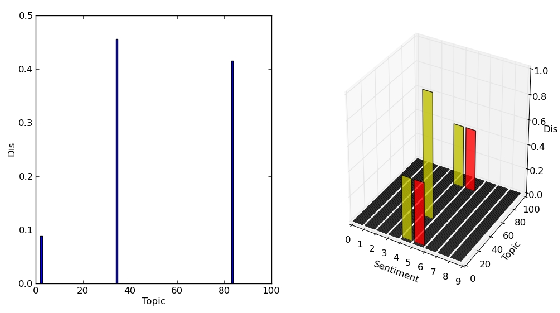
\includegraphics[width=3.3in,height=1.2in]{fig1.pdf}
\caption{Subjectivity model of user $u$. The left subgraph denotes interests distribution on topic 2, 32 and 83: $ (  w_{u,2}=0.08,w_{u,32}=0.48, w_{u,83}=0.44)  $. The right subgraph denotes opinions towards topics: $ O_{2}=( d_{u,2,4} =0.5, d_{u,2,5} =0.5)$, $O_{32}=(d_{u,32,4}=1.0) $, $ O_{83}=( d_{u,83,4}=0.5, d_{u,83,5}=0.5 ) $.}
\label{fig0}
\end{figure}
%The definition of the subjectivity model is in an abstract form, which needs to be concreted from two aspect:(1)how to construct the subjectivity model (2)how to utilize this model for retweeting analysis.
 
\subsection{Establishment of Subjectivity Model}
\label{establishment}

In this section, we present our framework of how to concrete subjectivity model by deriving topics and opinions from the UGC of users $ M=\lbrace M_{u}\vert u \in V\rbrace$.

\subsubsection{Topic Analysis}
\label{topic}

%We simply use the concept of topics to broadly refer to the different kinds of content such as key words, entities, hashtag, etc. 
Previous studies have tried to identify topics from tweets by finding key words\cite{chen2010short}, extracting  entities\cite{abel2011analyzing} or linking tweets to external knowledge categories\cite{macskassy2011people}. However, works show that topic model is more effective in identifying topics from short and informal social media language\cite{hong2010empirical}. In this paper, state-of-the-art Latent Dirichlet Allocation (LDA)\cite{blei2003latent} is employed for unsupervised topic discovery and for topic assignment of future tweets. LDA can be used to find a set of $ K $ latent topics from a document corpus, and then to represent each document $ D $ with a distribution $ \theta_{D} $ of the latent topics. For each word $ w_{i} $ in $ D $, a topic $ z $ is first sampled from the document topic distribution $ \theta_{D} $, then $ w_{i} $ is sampled according to word distribution $ \phi_{z} $ of topic $ z $. 

As the first step, we adopt the user-level LDA model to build a global Topic Model (TM), which takes all tweets of a user $M_u$ as one document of LDA\cite{hong2010empirical}. The TM model will be used throughout our framework. 
%For a single tweet $ t $, each dimension $ i $ of its topic distribution $ \theta_{t} $ can be obtained as follows:
%\begin{equation}
%\theta_{t,i}=\dfrac{\prod_{w \in t}P(w|\phi_{i})}{\prod_{w \in t}\sum_{k}P(w|\phi_{k})}
%\end{equation}
Usually a tweet concentrates on a single topic within its short length, therefore we assign a tweet $ t $ to a topic that maximizes the probability of generating $ t $:
\begin{equation}
\label{twtopic}
z_{t} = \arg \max_{k}\prod_{w \in t} P(w|\phi_{k})
\end{equation}
We can get a weight distribution on each topic $ k $ of user $ u $ by normalizing all tweets that talk about topic $ k $: 
\begin{equation}
w_{u,k}=\dfrac{|\{ t: t \in M_{u} \wedge z_{t}=k\}|}{|M_{u}|}
\end{equation}

\subsubsection{Opinion Analysis}
\label{opinion}

%Most previous opinion mining researches\cite{liu2012sentiment} represent opinion with a porlarity label in a binary sentiment space (0, 1): 1 means opinion agreement or positive sentiment, 0 means opinion disagreement or negative sentiment. However, such approach cannot fully distinguish user's detail opinion. 
Considering the example in Figure~\ref{fig00}, both Tony and Jane held an overall positive opinion on the movie ``Frozen'', but maybe they liked the movie for different reasons. Jane maybe mainly liked the romantic story of this movie but was a little disappointed at its animation picture, while Tony liked this movie perhaps because he was mostly convinced by its animation technology although he disliked the prince and princess genre. Previous works usually represent opinion with a simple binary polarity, without differentiating opinions on different aspects, thus they may not satisfy the information discovery needs of different users. Therefore, it is better to describe opinion for a topic as a probability distribution over the sentiment space. Furthermore, a more fine-grained sentiment space is preferred if we want to distinguish subjectivities of users more precisely.

Researches on sentiment analysis of social media have provided many effective state-of-the-art techniques and tools\cite{thelwall2010sentiment,hu2013unsupervised}, with which sentiment of a tweet $ t $ can be identified as $ s_t $. The opinion distribution $ O_k $ toward a topic $ k $ can be integrated as:
\begin{eqnarray}
O_k &= & \{ d_{u,k,s}|s \in S \} \nonumber \\
  &=& \{ \dfrac{|t:t \in M_u \wedge z_t=k \wedge s_t=s|}{|M_u|}|s \in S\}
\end{eqnarray}

\subsection{Subjectivity Similarity}
\label{similarity}

With the subjectivity model established, a subjectivity similarity measurement needs to be calculated to analyze various subjective decision-making processes such as retweeting behavior. 
Firstly we should define the opinion similarity on a common topic. 
 
\subsubsection{Opinion Similarity}
\label{opsim}

Opinion in the subjectivity model is treated  as a distribution over sentiment space with each dimension of the distribution representing the proportion of the corresponding sentiment value. 
In fact, values of the sentiment space are not independent. 
They are sequential in magnitude and quantified to measure the strength of sentiment. Therefore, normal distribution similarity measurements such as KL-divergence and cosine similarity are not suitable for such kind of opinion distribution. As illustrated in Table~\ref{tab1}, in a $ S=[0,8 ] $ integer sentiment space, opinion $ O_{k}^{1} $ is most negative (100\% of value 0), opinion $ O_{k}^{2} $ (50\% of value 6 and 50\% of value 7) is positive, and $ O_{k}^{3} $ (100\% of value 8) is most positive.
If the cosine similarity measurement is adopted, all similarities among them are 0.
In fact $ O_{k}^{2} $ is more similar to $ O_{k}^{3} $ than $O_{k}^{1} $ because they both are positive and their strength distance is much less than $ O_{k}^{1} $.  
Therefore, opinion similarity can't be calculated simply as normal probabilistic distributions, or just as strength distance. 
To accurately catch opinion similarity, we propose a novel method by combining strength distance and distribution similarity.
The opinion similarity between two opinions $O_{k}^{u},O_{k}^{v} $on the same topic $ k $ can be calculated as: 
\begin{equation}
\label{opinionsim}
Sim(O_{k}^{u},O_{k}^{v})=\dfrac{|S|-|\sum_{i=0}^{|S|}d_{i}^{u}v_{i}-\sum_{i=0}^{|S|}d_{i}^{v}v_{i}|}{|S|}
\end{equation}
where $ d_{i} $ denotes the $ i^{th} $ dimension of opinion distribution, and $ v_{i} $ denotes corresponding sentiment value. 
\begin{table}[htb]
\scriptsize
\centering
\caption{Illustration of opinion similarity}
\label{tab1}
\begin{tabular}{|l|l|l|l|l|l|l|l|l|l|}
\hline
 & 0 & 1& 2 & 3 & 4 & 5 & 6 & 7 & 8 \\
\hline
$O_{k}^{1}$ & 1.0 & 0.0 & 0.0 & 0.0 & 0.0 & 0.0 & 0.0 & 0.0 & 0.0 \\
\hline
$O_{k}^{2}$ & 0.0 & 0.0 & 0.0 & 0.0 & 0.0 & 0.0 & 0.5 & 0.5 & 0.0 \\
\hline
$O_{k}^{3}$ & 0.0 & 0.0 & 0.0 & 0.0 & 0.0 & 0.0 & 0.0 & 0.0 & 1.0 \\
\hline
\end{tabular}
\end{table} 
The similarities of opinions in Table~\ref{tab1} calculated with Equation~\ref{opinionsim} are $ Sim(O_{k}^{1},O_{k}^{3})=0 $, $ Sim(O_{k}^{2},O_{k}^{3})=6/8 $ and $ Sim(O_{k}^{1},O_{k}^{2})=2/8 $, which are consistent with our intuitive understanding. 

\subsubsection{Subjectivity Similarity}

As the subjectivity model indicates, a user's topics of interest is represented as a weight distribution over topic space $ T $. Therefore, the subjectivity similarity between two subjecctivity models $SM_u$ and $SM_v$ should be integrated by combining the topic weight and the opinion similarity on each common topic:
\begin{equation}
\label{subsim}
Sim(SM_{u},SM_{v})=\sum_{k=1}^{|T_{u,v}|}\theta_{u}(k)\* Sim(O_{k}^{u},O_{k}^{v})
\end{equation}
Where $ T_{u,v} $ denotes the common topics between two users, which can be regarded as the intersection of their topics of interest; $ \theta_{u}(k) $ denotes the weight of topic $ k $ of user $ u $.

Note that, when we measure how similar user $ u $ is to user $ v $, we use the topic weight of user $ u $, thus the subjectivity similarity is asymmetric. The intuition lies in that subjectivity of a user is a personal inner taste, and it is also one-way judgement about how like-minded a friend is. Therefore, for the measurement of subjectivity similarity, $ Sim(SM_u,SM_v)\neq Sim(SM_v,SM_u)$.

\section{Retweeting Analysis}
\label{retweet}

Whether a user retweets a message may be affected by various factors. 
%As a user mainly uses Twitter as source of information, a tweet is more likely to be retweeted because the user finds its content worth to. 
From the point of a user, three situations usually make him rewteet: 1) the content of the tweet is attractive for the user, and his retweeting behavior is in accordance with subjective evaluation; 2) the tweet is posted by the user's close friend, and his retweeting behavior is due to social needs; and 3) the content is popular, and his retweeting behavior is a result of conformity needs\cite{cialdini2004social}. These situations exhibit different types of reasons of rewteeting behavior, and we quantify them with three subjectivity similarities for the motivation analysis in our work. 
For a target tweet $ t $, let $ F $ denote the followers who receive $ t $ by following its author $ u_{a} $. 
For each follower $ f \in F $, we can define a quadruple $ <f, u_{a}, t, r_{f}>  $, where $ r_{f} $ is a binary label indicating if $ t $ is retweeted by $ f $, which needs to be predicted.

\subsection{Attractiveness}

A user is likely to repost a tweet if the user finds the content is attractive according to his subjective judgement. We can measure such attractiveness quantitatively by calculating the subjectivity similarity between the tweet $ t $ and user $ f $. For a tweet $ t $, its topic $ z_t $ can be identified with Equation~\ref{twtopic}, and let $ s_t $ be its sentiment. The content of $ t $ can also be modeled using subjectivity model definition with a single topic of interest and a 100\% opinion distribution on sentiment value $s_t$. Thus the attractiveness of tweet $t$ to user $f$ can be measured with subjectivity similarity using Equation~\ref{subsim}, which is marked as $ Sim(f,t) $.

\subsection{Sociality}

In this case, the retweeting behavior is based on the needs of social interaction. That is, the behavior is triggered because the tweet is sent by a like-minded friend, instead of the information it contains. We can measure how like-minded the user $ f $ and his friend $ u_a $ are with their subjectivity similarity $ Sim(f,u_a) $.  However, different kinds of friends may have a different influence on the user $ f $. For example, $ f $ may follow many friends, but only frequently interacts with a few. Furthermore, not all tweets of a friend may be of interest to $ f $. For example, in Figure~\ref{fig00}, Jane may be interested in the tweets from Tony about movie, but not interested in his tweets about cellphone. We therefore assign a weight to $ Sim(f,u_a) $ to reflect the influence of different kinds of friend, which
is composed of four factors:
\subsubsection{Expert Factor $ w_E(u_a) $:} It represents the relative expertise of the author $ u_a $ among his followers including $ f $. The expert user imposes more influence on others. We simply calculate it as the ratio of user $ u_a $'s tweets count over all tweets of $ u_a $ and his followers by $ w_E(u_a)=|M_{u_a}|/|\{M_u|u \in u_a \cup F \}|  $.
\subsubsection{Leadership Factor $ w_L(u_a) $:} In our work, the leadership of a user $ u_a $ is determined by his followers. The leadership weight is calculated by $ w_L(u_a)=\log (|F|)/\log(\max) $, where $ \max $ is the maximum popularity of a user in Twitter\footnote{\url{http://twittercounter.com/pages/100}}.
\subsubsection{Similarity Factor $ w_S(u_a,f) $:} The similarity of interests between $ u_a $ and $ f $ is measured as the inverse KL-divergence between their topic weight distribution in their subjectivity model: $ w_S(u_a,f)= 1/KL(\theta_{u_a},\theta_f)$.
\subsubsection{Interaction Factor $ w_I(u_a,f) $:} All the interactions $ Interation_{u_a,f} $ between $ u_a $ and $ f $ are analyzed, which include the conversations between them, mentions of each other, and retweets from each other. The factor weight is calculated by normalizing $Interation_{u_a,f}$ with all tweets of $ u_a $ and $ f $: $ w_I(u_a,f)=|Interation_{u_a,f}| /|\{ M_{u_a}, M_f \}| $.

Above all, the influence weight is the combination of four factors:
\begin{equation}
\begin{split}
w_{u_a,f}=& \lambda_1*w_E(u_a)+\lambda_2*w_L(u_a)+\\
   &\lambda_3*w_S(u_a,f)+\lambda_4*w_I(u_a,f). 
\end{split}
\end{equation}
where $ \lambda_i $ is an optional weight vector to enable different influence of the factors,  subject to $ \sum_{i=1}^{4}\lambda_i=1 $. We set them uniformly as 0.25 in our work.

\subsection{Popularity}

If a tweet is popular(novel or epidemic), it will be very probable to be retweeted. In this situation, the tweet $ t $ is often inconsistent with the interests and opinions of its author $ u_a $. Thus the similarity between $ t $ and $ u_a $ in terms of subjectivity is relatively low, which is marked as $ Sim(u_a,t) $. The retweeting behavior is highly related to the popularity of $ t $ rather than the content or the friend who post it. We assign a popularity weight to $ Sim(u_a,t) $, which is the proportion of user $ f $'s followees who have retweeted the tweet $ t $.

From the point of motivation, a user might retweet a message if its content is approximate to his subjectivity, its author is a like-minded friend or it is popular among his friends. 
%In next section a set of experiments are carried out to verify the impact of such motivation on retweeting behavior. 

\section{Experiments}
\label{experiments}

\subsection{Dataset and Settings}
Our method has been evaluated on the Twitter dataset from \cite{Luo:2013RMF}, in which 500 target English tweets were monitored to find who would retweet it in the future. 
Each target tweet was set as starting point to collect recent tweets for its author and followers.
Overall, there are 45,531 users who have posted at least 6,277,736 tweets. 5214 users have retweeted at least one target tweet during the monitored period. To avoid the bias introduced by dataset imbalance, an evaluation dataset is constructed by taking 5,214 retweeters as positive instances, and randomly sampling 5,214 non-retweeters as negative instances. 

For the topic model, we use Gensim\cite{rehurek_lrec}, which adopts an efficient batch-based online inference algorithm. All parameters are set as defaults and the number of topic traverses from 50 to 200. For sentiment analysis, we just make use of an off-the-shelf work, i.e. SentiStrength\cite{thelwall2010sentiment}. In order to catch the sentiment of tweets, we use the sentiment lexicon created based on AFINN by Nielsen\cite{MohammadKZ2013}. The sentiment space is formed by mapping the positive and negative sentiment values to range $ [0,8] $.

\subsection{Correlation Test}

First of all we assess the correlation between subjectivity similarity and retweeting behavior with a statistical hypothesis test Analysis of Variance (ANOVA)\cite{fisher1970statistical}, which tests the \textit{null hypothesis} that the retweeters and non-retweeters have the same subjectivity similarity means. 
The results are listed in Table~\ref{tab2}. The bold-faced entries mean that the \textit{p-value} is lower than significance level.
\begin{table}[htb]
\scriptsize
\centering
\caption{ANOVA results for subjectivity similarities. If the difference is due to chance, \textit{F-ratio}=1.00, otherwise \textit{F-ratio} \textgreater 1.00 (\textit{p-value} \textless 0.01).}
\label{tab2}
\begin{tabular}{|c|c|c|c|c|}
\hline
\multicolumn{2}{|c|}{Similarity}& $ Sim(f,t) $ & $ Sim(f,u_a)  $ & $ Sim(u_a,t)  $\\
\hline
\multirow{2}{*}{50} & \textit{F} & \textbf{12.182} & 2.212 & 4.236 \\
\cline{2-5}
  & \textit{p} &  $\mathbf{4.44e^{-06}}$  & 0.140 & 0.272\\
\hline
\multirow{2}{*}{100} & \textit{F} & \textbf{43.892} & \textbf{31.145} & \textbf{28.466} \\
\cline{2-5}
  & \textit{p} &  $\mathbf{8.65e^{-11}}$  & $\mathbf{3.55e^{-08}}$ & $\mathbf{1.32e^{-09}}$\\
\hline
\multirow{2}{*}{150} & \textit{F} & \textbf{22.356} & \textbf{12.240} & \textbf{14.664} \\
\cline{2-5}
  & \textit{p} &  $\mathbf{2.43e^{-08}}$  & $\mathbf{6.25e^{-06}}$ & $\mathbf{8.46e^{-07}}$\\
\hline
\multirow{2}{*}{200} & \textit{F} & \textbf{31.675} & \textbf{20.616} & 6.145\\
\cline{2-5}
  & \textit{p} &  $\mathbf{4.22e^{-06}}$  & $\mathbf{2.92e^{-05}}$ & 0.26\\
\hline
\end{tabular}
\end{table}
Note that for the topic numbers of 100 and 150, all similarities yield \textit{p-values} below significance level with \textit{F-ratio} above 1.00. This suggests that the subjectivity similarities could be useful features for modeling retweeting behavior. 
For the rest experiments, we set the topic number as 100 for LDA. 

\subsection{Case Study}
\label{example}
In this section, we give an vivid example to illustrate the subjectivity model and its ability in explaining the retweeting behavior. 
The subjectivity models of one of the 500 target tweets, its author, and two followers (one retweeter, the other non-retweeter) are shown in Figure~\ref{fig5}. 
The right part of each sub-figure illustrates topic distribution and the left part illustrates opinions on each topic. 
\begin{figure*}[htb]
\centering
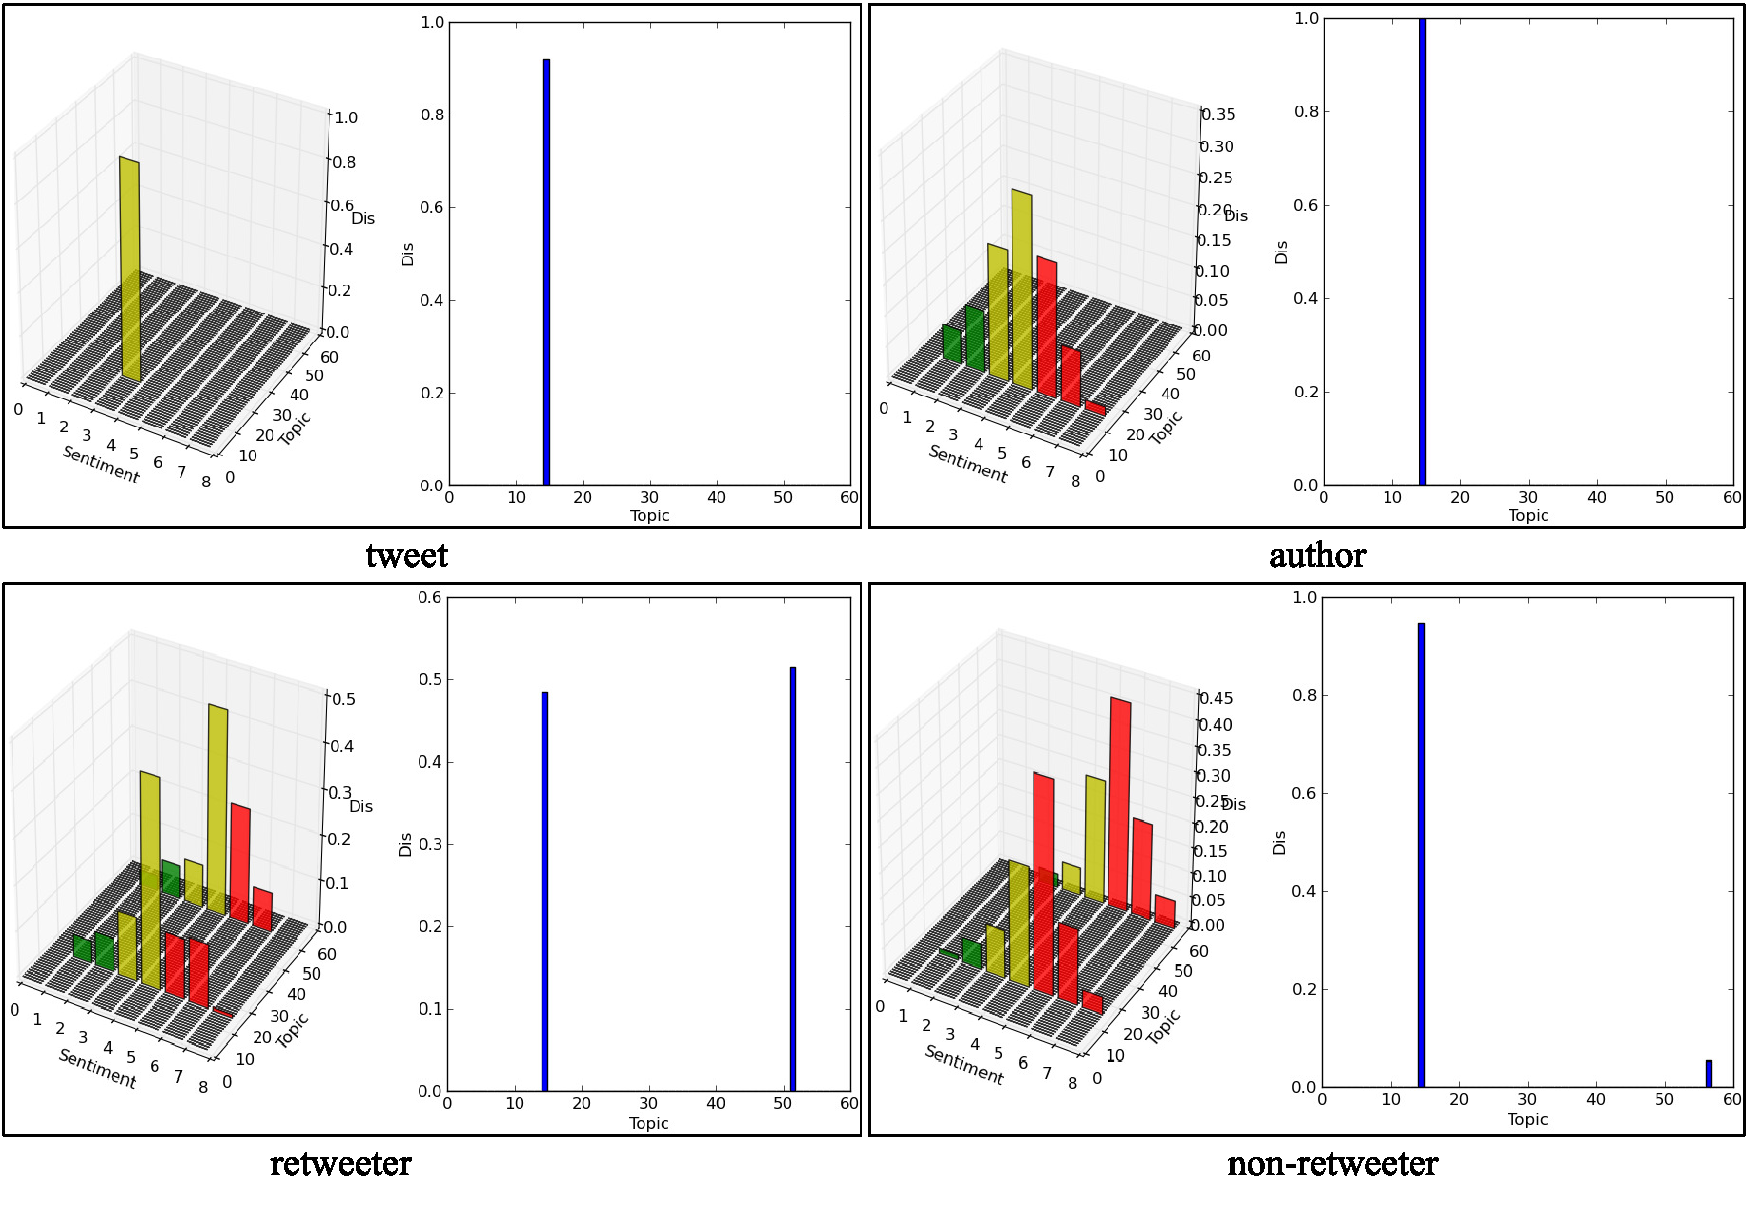
\includegraphics[width=4.5in,height=2.5in]{fig5.pdf}
\caption{An illustration of subjectivity models of a tweet, author and two followers.}
\label{fig5}
\end{figure*}

It is obvious that the tweet is about the $ 14^{th} $ topic, and the opinion is neutral.
The author concentrates on the $ 14^{th} $ topic, and his opinion is mainly neutral.
% ($O_{u_{a}}^{14} =( 0, 0.04, 0.05, 0.25, 0.35, 0.25, 0.05,  0.01 )$). 
As for two followers, the retweeter has tweeted on two topics (the $ 14^{th} $ and $ 52^{nd} $ topic) uniformly 
%(with $ w_{u_{r}}(14)=0.48 $) 
and his opinion on the $ 14^{th} $ topic is mainly neutral.
%($O_{u_{r}}^{14} =( 0, 0.02, 0.04, 0.15, 0.50, 0.13,  0.15,  0.01)$). 
While the non-retweeter has also talked about two topics ($ 14^{th} $ and $ 56^{th} $ topic), but he is mainly interested in the $ 14^{th} $ topic 
%(with $ w_{u_{n}}(14)=0.98 $) 
and his opinion is positive.
% ($O_{u_{n}}^{14} =( 0, 0.01, 0.04, 0.10, 0.25, 0.45, 0.13, 0.02)$).

Table~\ref{tab4} shows the three subjectivity similarities for both retweeter and non-retweeter. It is clear that except for the similarity between the tweet and its author, the other two subjectivity similarities of the retweeter are much larger than the non-retweeter.
\begin{table}[h]
\scriptsize
\centering
\caption{ Illustration of example subjectivity similarities}
\label{tab4}
\begin{tabular}{|c|c|c|c|}
\hline
Similarity & $ Sim(f,t) $ & $ Sim(f,u_a)  $ & $ Sim(u_a,t)  $\\
\hline
Retweeter & 0.854 & 0.967 & 0.886\\
\hline
Non-retweeter & 0.805 & 0.919 & 0.886\\
\hline
\end{tabular}
\end{table} 
They have common interest (the $ 14^{th} $ topic), and furthermore the non-retweeter is more similar with the tweet and its author than the retweeter in terms of topics. But their different opinions towards the topic elicit their different behaviors, which verifies our model can help better understanding the retweeting behavior not only from topics but also opinions.

\subsection{Performance Evaluation}

We carried out the retweeting prediction experiments in three stages. Firstly we compared our model against other topic-based models including TF-IDF model (modeling user interests using bag-of-words), entity-based model (using entities extracted from the UGC) and hashtag-based model (using hashtags used in the UGC)\cite{abel2011analyzing}.
Secondly, our model was compared with two generative topic-sentiment models (TSM model\cite{mei2007topic} and JST model\cite{lin2009joint}). TSM and JST can also model topic and topic related sentiment simultaneously. We also use Equation~\ref{subsim} to calculate three  subjectivity similarities for bith TSM and JST as our method in section~\ref{retweet}, and combine them together in the predction.

The subjectivity model has been proposed to catch the subjective motivation of users based on UGC, whereas other important factors associated with retweeting behavior are not considered, such as network topology and meta-data of users. 
Therefore, our model is also compared with the method of Luo \emph{et al.}~\shortcite{Luo:2013RMF}(marked as ``LUO''), in which different factors that might affect rewteeting behaviors are considered.
They only use bag-of-words to model user interests, so we also carried out combining experiments to demonstrate that the performance of prediction can be improved by replacing their bag-of-words model with our model (marks with ``LUO+'' prefix). 
\begin{table}[htb]
\scriptsize
\centering
\caption{Accuracy performance. A significant improvement over baseline with $ \ast $ and LUO's model with $ \ddagger $ ($p < 0.05$).}
\label{tab3}
\begin{tabular}{|l|l|l|l|}
\hline
Feature & Accuracy(\%) & Feature & Accuracy(\%)\\
\hline
baseline & 60.85 & & \\
\hline
TF-IDF & 62.85   $\ast$ & LUO & 71.76 $ \ast  $\\
entity & 68.76  $\ast$ & LUO+entity & 72.15 $\ast$\\
hashtag & 59.12  & LUO+hashtag & 68.44 $\ast$\\
\hline
TSM & 67.44 $\ast$ & LUO+TSM & 68.23 $\ast$\\
JST & 68.13 $\ast$ & LUO+JST & 70.53 $\ast$\\
\hline
$ Sim(f,t) $ & 73.88   $\ast  \quad \ddagger $ &LUO+$ Sim(f,t)$ & 74.04  $ \ast \quad \ddagger $\\
$ Sim(f,u_a)  $ & 70.04   $\ast  $ & LUO+$ Sim(f,u_a)$ & 70.27  $ \ast $\\
$ Sim(u_a,t)  $ & 69.64   $\ast  $ & LUO+$ Sim(u_a,t)$ & 71.86  $ \ast $\\
$ sim_{all}  $ & \textbf{75.64}   $\ast \quad \ddagger $ & LUO+$ sim_{all}  $ & \textbf{78.15}  $ \ast \quad \ddagger $\\
\hline
\end{tabular}
\end{table}

The logistic regression classifier is used for training and testing in a 5-fold cross-validation manner.
We set a baseline, which simply predicts users who have retweeted the author previously as the retweeters of target tweet. 
All results are presented in Table~\ref{tab3} in terms of accuracy.

Firstly, all models except the hashtag-based model outperform the baseline (60.85\%) significantly. While for hashtag-based model, the accuracy is only 59.12\%, the reason lies in the sparcity of hashtag in tweets. 

Secondly, $ Sim(f,t) $ and $ sim_{all}  $ outperform ``LUO'' (71.76\%) significantly.
The best performance is achieved by the $ sim_{all}  $ (75.64\%), for which we add three similarities to the classifier to test the impact of their combination. 
The performance of TF-IDF model (62.85\%) is a little better than baseline. 
The entity-based model (68.76\%) is very close to  $ Sim(f,u_a)$ (70.04\%) and $ Sim(u_a,t)  $ (69.64\%), and the difference is not significant.

Thirdly, the performance of two topic-sentiment models (TSM: 67.44\%, JST: 68.13\%) is not as good as our models. The reason lies in that they use a binary sentiment representation (positive or negative), which can not differentiate opinions elaborately. Our model can capture more subtle and fine-grain sentiment, which could distinguish different subective motivation of retweeting behavior.

Finally, in the combining evaluation, $ Sim(f,t) $ gives a significant improvement (LUO+$ Sim(f,t) $, 2.12\% improvement) over ``LUO'', but other two similarities and the entity-based model can not improve performance significantly. The performance is even degraded after combining with the hashtag-based model and two topic-sentiment models. 
But noticing that, the most significant improvement(LUO+$ sim_{all}  $, 6.39\% improvement) is achieved by combining with all three similarities. 

Above all, the results show that our model can better help predicting retweeting behavior and can be regarded as a useful way to analyze the retweeting behaviors of users. 

\section{Conclusion}
Motivated by the psychological research, this paper postulates that the diffusion behaviors of social media users are affected by their subjectivity. Therefore, a general subjectivity model has been proposed and an efficient framework has been designed to establish the subjectivity model. Also a novel method is proposed to measure the subjectivity similarity. The subjectivity model has been applied to the retweeting analysis considering the attractiveness, sociality and popularity factors, which are quantified with subjectivity similarities. 
Experiment results demonstrate the effectiveness of the proposed model in the retweeting analysis problem and show that the model is able to reach better understanding of retweeting behavior. 
In the future, we will apply our model to other social network analysis task such as link prediction and recommendation. 

\bibliography{subjectivity}
\bibliographystyle{aaai}
\end{document}
